
\item A shell acquires the initial velocity \(v = 320 \, \text{m/s}\), having made \(n = 2.0\) turns inside the barrel whose length is equal to \(l = 2.0 \, \text{m}\). Assuming that the shell moves inside the barrel with a uniform acceleration, find the angular velocity of its axial rotation at the moment when the shell escapes the barrel.
    \begin{center}
        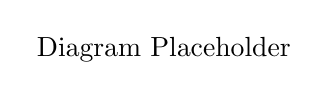
\begin{tikzpicture}
            %% Code for the actual diagram would go here. Replace the text with the corresponding TikZ commands.
            \node at (0, 0) {Diagram Placeholder};
        \end{tikzpicture}
    \end{center}

\begin{solution}
    \begin{center}
        \begin{tikzpicture}
            \pic at (0, 0) {frame=3cm};
        \end{tikzpicture}
    \end{center}
    
    \begin{align*}
        \intertext{The shell acquires a constant angular acceleration at the same time as it accelerates linearly.}
        l &= \dfrac{1}{2}wt^2 \quad \text{and} \quad 2\pi n = \dfrac{1}{2}\beta t^2\\
        \intertext{So,}
        \dfrac{w}{l} &= \dfrac{\beta}{2\pi n}\\
        \intertext{(where \( w = \) linear acceleration and \( \beta = \) angular acceleration).}
        \omega &= \sqrt{2\beta 2\pi n} = \sqrt{\dfrac{2w}{l}(2\pi n)^2}\\
        \intertext{But,}
        v^2 &= 2wl\\
        \intertext{Hence,}
        \omega &= \dfrac{2\pi nv}{l} = 2.0 \times 10^3 \text{ rad/s} \quad \text{(on substituting values)}
    \end{align*}
\end{solution}
